\documentclass{article}
\usepackage{graphicx}
\usepackage{adjustbox}
%\usepackage{astron}
\usepackage{natbib}
\usepackage{hyperref}
\usepackage{xurl}
\usepackage{geometry}
\usepackage{amsmath}
\usepackage{booktabs}
\geometry{margin=1in}
\usepackage{fancyhdr}
\usepackage{setspace}
\usepackage{lipsum} % For placeholder text, can be removed
\usepackage{listings}
\usepackage{xcolor}

% Define MATLAB style for listings
\lstdefinestyle{MatlabStyle}{
	language=Matlab,
	basicstyle=\ttfamily\footnotesize,
	keywordstyle=\color{blue},
	stringstyle=\color{red},
	commentstyle=\color{green!50!black},
	numbers=left,
	numberstyle=\tiny\color{gray},
	stepnumber=1,
	numbersep=5pt,
	backgroundcolor=\color{white},
	showspaces=false,
	showstringspaces=false,
	showtabs=false,
	frame=single,
	tabsize=2,
	captionpos=b,
	breaklines=true,
	breakatwhitespace=false,
	escapeinside={\%*}{*)}
}

\begin{document}
	
	\begin{titlepage}
		\thispagestyle{empty}
		\pagenumbering{Roman}
		\frenchspacing
		
		\noindent
		\begin{tabular}{@{} c @{\hspace{0.1cm}} c @{\hspace{0.2cm}} c @{}}
			% Adjust and include the first image
			\adjustbox{valign=c}{%
				
\includegraphics[height=2cm, trim=0 0 0 0, clip]{sedes.pdf}%
			} &
			% Add the vertical black line
			\adjustbox{valign=c}{%
				\rule{0.5pt}{2cm}%
			} &
			% Adjust and include the second image
			\adjustbox{valign=c}{%
				
\includegraphics[height=2cm, trim=0 0 0 0, clip]{logoFirW.jpg}%
			}
		\end{tabular}
		\hfill
		
		\vspace*{2cm}
		
		\begin{center}
			\begin{minipage}[t]{\textwidth}
				\begin{center}
					\large\textbf{B-KUL-H04X3A: Control Theory}
				\end{center}
				\vspace{1cm}
				\begin{center}
					\textbf{Team members:}\\[2mm]
					Lefebure Tiebert (r0887630)\\
					Campaert Lukas (r0885501)\\
				\end{center}
				\vspace{1cm}
				\begin{center}
					\Huge\textbf{Assignment 1: Identification of the Cart}
				\end{center}
				\vspace{1cm}
				\begin{center}
					\underline{Professor:}\\[2mm]
					Prof. Dr. Ir. Jan Swevers\\
				\end{center}
				\vspace{2cm}
				\makebox[\textwidth]{Academic Year 2025-2026}
			\end{minipage}
		\end{center}
	\end{titlepage}
	
	\newpage
	
	\vspace*{3.2cm}\vfill
	
	\begin{center}
		\Large\textbf{\textit{Declaration of Originality}}
	\end{center}
	
	\noindent \textit{We hereby declare that this submitted draft is entirely our own, subject to feedback and support given us by the didactic team, and subject to lawful cooperation which was agreed with the same didactic team. Regarding this draft, we also declare that:}
	
	\begin{enumerate}
		\item \textit{Note has been taken of the text on academic integrity \url{https://eng.kuleuven.be/studeren/masterproef-en-papers/documenten/20161221-academischeintegriteit-okt2016.pdf}.}
		\item \textit{No plagiarism has been committed as described on \url{https://eng.kuleuven.be/studeren/masterproef-en-papers/plagiaat\#Definitie:\%20wat\%20is\%20plagiaat?}.}
		\item \textit{All experiments, tests, measurements, \ldots, have been performed as described in this draft, and no data or measurement results have been manipulated.}
		\item \textit{All sources employed in this draft – including internet sources – have been correctly referenced.}
	\end{enumerate}
	
	\newpage
	
	\section{Discrete-time model structure selection}
	
	To select an appropriate model structure for identifying the relation between motor voltage and rotational wheel velocity, we start by analyzing the continuous-time dynamics of the DC motor, incorporating the following assumptions:
	
	\begin{itemize}
		\item the same voltage is applied to both motors
		\item no wheel slip occurs
		\item only forward and backward motions are considered (no turning)
		\item the cart's mass and ground friction are lumped into the wheel inertia and friction respectively
	\end{itemize}
	
	\noindent When Laplace transforming the equations in our lumped model (see Figure~\ref{fig:dc_motor_model} in Appendix~\ref{app:figures}) of conservation of momentum and charge, and working out towards $\dot{\Theta}_m(s)/V_a(s)$, one obtains the following transfer function:
	
	\begin{equation}
		H(s) = \frac{\dot{\Theta}_m(s)}{V_a(s)} = \frac{K}{(J_ms + b)(L_as + R_a) + K^2} 
		\label{eq: CT transfer function DC}
	\end{equation}
	
	\begin{table}[htbp]
		\centering
		\label{tab:laplace_variables}
		\begin{tabular}{@{}ll@{}}
			\toprule
			\textbf{Symbol} & \textbf{Description} \\ \midrule
			\( \dot{\Theta}_m(s) \) & Laplace transform of the angular velocity $\dot{\theta}_m$ \([ \text{rad/s} ]\)  \\
			\( V_a(s) \) & Laplace transform of the applied voltage $v_a$ \([ \text{V} ]\) \\
			\( J_m \) & moment of inertia of the rotor \([ \text{kg\,m}^2 ]\) \\
			\( b \) & damping coefficient (viscous friction) \([ \text{N\,m\,s/rad} ]\) \\
			\( K \) & motor torque and back EMF constant \([ \text{N\,m/A} ]\) or \([ \text{V\,s/rad} ]\) \\
			\( L_a \) & armature inductance \([ \text{H} ]\) \\
			\( R_a \) & armature resistance \([ \Omega ]\) \\
			\bottomrule
		\end{tabular}
	\end{table}
	
	\noindent This continuous-time transfer function relates the input voltage \( v_a(t) \) to the rotational speed of the motor shaft \( \dot{\theta}_m(t) \). We can represent the transfer function with generic coefficients since the exact values of the physical constants are unknown and will be estimated later. Therefore, \( H(s) \) becomes:
	\begin{equation}
		H(s) = \frac{\dot{\Theta}_m(s)}{V_a(s)} = \frac{a}{bs^2+cs+d} 
	\end{equation}
	

	
	\subsection{Discrete-time transfer function}
	
	The discrete-time transfer function with computational delay is:
	\begin{equation}
		H(z) = \frac{b_1 z + b_2}{z^{3} + a_1 z^{2} + a_2 z}
	\end{equation}
	This is a third-order model with numerator order 1, denominator order 3, and relative order 2 (indicating two delays: one from motor dynamics and one from microOS latency).
	
	\subsection{Model derivation}
	
	The discrete-time model was derived by applying Zero-Order Hold (ZOH) discretization to the continuous-time transfer function using MATLAB's \texttt{c2d} function. The one-sample delay ($z^{-1}$) was added to account for computational latency in the microOS embedded system. This yields the transfer function above with four unknown parameters ($a_1, a_2, b_1, b_2$) to be estimated from experimental data.
	
	\subsection{Model structure motivation}
	
	We consider two model structures: (1) the full third-order model above, which captures armature inductance effects, and (2) a simplified second-order model neglecting inductance ($L_a$), yielding $H(z) = \frac{b_1}{z^2 + a_1 z}$ with only two parameters. The third-order model is selected as the primary structure because it preserves more of the physical dynamics. The second-order model serves as a simplified alternative if parameter estimation reveals that inductance effects are negligible.
	
	\section{Model parameters estimation}
	
	\subsection{Armature inductance \texorpdfstring{$L_a$}{La} included (third-order \texorpdfstring{$H(z)$}{H(z)})}
	
	\subsubsection*{Recursion expression}
	
	To estimate the model parameters ($a_1, a_2, b_1, b_2$) of the discrete-time transfer function, we employ an Auto-Regressive with eXogenous input (ARX) model structure. The transformation from the transfer function to a recursion expression (difference equation) proceeds as follows:
	
	Starting from the discrete-time transfer function:
	\[
	H(z) = \frac{\dot{\Theta}(z)}{V(z)} = \frac{b_1 z + b_2}{z^3 + a_1 z^2 + a_2z}
	\]
	
	Cross-multiplying yields:
	\[
	(z^3 + a_1z^2 + a_2z)\dot{\Theta}(z) = (b_1z + b_2)V(z)
	\]
	
	Dividing both sides by $z^3$ to express in terms of the delay operator $z^{-1}$:
	\[
	(1 + a_1z^{-1} + a_2z^{-2})\dot{\Theta}(z) = (b_1z^{-2} + b_2z^{-3})V(z)
	\]
	
	Applying the inverse Z-transform (where $z^{-k}$ corresponds to a delay of $k$ samples) gives the difference equation:
	\begin{equation}
		\dot{\theta}[k] + a_1\dot{\theta}[k-1] + a_2\dot{\theta}[k-2] = b_1 v[k-2] + b_2 v[k-3]
		\label{eq: difference eq}
	\end{equation}
	
	Rearranging to express the current output as a function of past outputs and inputs:
	\begin{equation}
		\dot{\theta}[k] = -a_1\dot{\theta}[k-1] - a_2\dot{\theta}[k-2] + b_1 v[k-2] + b_2 v[k-3]
		\label{eq: difference eq ARX}
	\end{equation}
	
	This linear difference equation represents an ARX model where the output $\dot{\theta}[k]$ depends linearly on:
	\begin{itemize}
		\item Two past output samples: $\dot{\theta}[k-1]$ and $\dot{\theta}[k-2]$ (auto-regressive terms)
		\item Two past input samples: $v[k-2]$ and $v[k-3]$ (exogenous input terms)
	\end{itemize}
	
	The ARX structure can be compactly written as:
	\begin{equation}
		\dot{\theta}[k] = \boldsymbol{\theta}^T \boldsymbol{\phi}[k]
		\label{eq: ARX form}
	\end{equation}
	
	where the parameter vector $\boldsymbol{\theta}$ contains all unknown model coefficients:
	\begin{equation}
		\boldsymbol{\theta} = \begin{bmatrix} a_1 \\ a_2 \\ b_1 \\ b_2 \end{bmatrix}
	\end{equation}
	
	and the regression vector $\boldsymbol{\phi}[k]$ contains the measured data at time step $k$:
	\begin{equation}
		\boldsymbol{\phi}[k] = \begin{bmatrix} -\dot{\theta}[k-1] \\ -\dot{\theta}[k-2] \\ v[k-2] \\ v[k-3] \end{bmatrix}
	\end{equation}
	
	Note that the negative signs in front of the output terms ensure consistency with the coefficient signs in equation~(\ref{eq: difference eq ARX}).
	
	\subsubsection*{Error criterion}
	
	The parameter estimation is based on the least squares (LS) criterion, which minimizes the sum of squared prediction errors. For each time step $k$, the prediction error is defined as:
	\[
	e[k] = \dot{\theta}[k] - \hat{\dot{\theta}}[k] = \dot{\theta}[k] - \boldsymbol{\phi}^T[k] \boldsymbol{\theta}
	\]
	
	where $\dot{\theta}[k]$ is the measured output and $\hat{\dot{\theta}}[k] = \boldsymbol{\phi}^T[k] \boldsymbol{\theta}$ is the model prediction.
	
	The least squares cost function to minimize over all $N$ measurements is:
	\begin{equation}
		V_N(\boldsymbol{\theta}) = \sum ^N _{k=1}  \frac{1}{2} [\dot{\theta}[k] - \boldsymbol{\phi}^T[k] \boldsymbol{\theta}]^2 = \frac{1}{2} \sum ^N _{k=1} e^2[k]
		\label{eq: LS criterion}
	\end{equation}
	
	The factor $\frac{1}{2}$ is included for mathematical convenience (it simplifies the derivative). This criterion seeks the parameter vector $\boldsymbol{\theta}$ that best fits the measured data in the least squares sense, i.e., $\hat{\boldsymbol{\theta}}^{LS}_N = \arg\min_{\boldsymbol{\theta}} V_N(\boldsymbol{\theta})$.
	
	\subsubsection*{Matrix formulation}
	
	For computational efficiency, the parameter estimation problem is formulated in matrix form. Consider all $N$ available measurements. Due to the delays in the difference equation (maximum delay is 3 samples), the prediction can only start from $k = 4$. 
	
	Define the output vector $\boldsymbol{y}$ as the $(N-3)$-dimensional column vector containing all valid output measurements:
	\begin{equation}
		\boldsymbol{y} = \begin{bmatrix}
			\dot{\theta}[4] \\ \dot{\theta}[5] \\ \vdots \\ \dot{\theta}[N]
		\end{bmatrix}
	\end{equation}
	
	Define the regression matrix $\boldsymbol{\Phi}$ as the $(N-3) \times 4$ matrix where each row is the transposed regression vector for the corresponding time step:
	\begin{equation}
		\boldsymbol{\Phi} = \begin{bmatrix}
			\boldsymbol{\phi}^T[4] \\
			\boldsymbol{\phi}^T[5] \\
			\vdots \\
			\boldsymbol{\phi}^T[N]
		\end{bmatrix} = \begin{bmatrix}
			-\dot{\theta}[3] & -\dot{\theta}[2] & v[2] & v[1] \\
			-\dot{\theta}[4] & -\dot{\theta}[3] & v[3] & v[2] \\
			\vdots & \vdots & \vdots & \vdots \\
			-\dot{\theta}[N-1] & -\dot{\theta}[N-2] & v[N-2] & v[N-3]
		\end{bmatrix}
	\end{equation}
	
	The least squares solution that minimizes equation~(\ref{eq: LS criterion}) is obtained by setting the gradient with respect to $\boldsymbol{\theta}$ to zero, yielding the normal equations. The solution is:
	\begin{equation}
		\hat{\boldsymbol{\theta}}^{LS}_N = [\boldsymbol{\Phi}^T \boldsymbol{\Phi}]^{-1} \boldsymbol{\Phi}^T \boldsymbol{y} = \boldsymbol{\Phi}^+ \boldsymbol{y}
		\label{eq: LS solution}
	\end{equation}
	
	where $\boldsymbol{\Phi}^+ = [\boldsymbol{\Phi}^T \boldsymbol{\Phi}]^{-1} \boldsymbol{\Phi}^T$ is the Moore-Penrose pseudo-inverse of $\boldsymbol{\Phi}$. This pseudo-inverse can be computed efficiently using singular value decomposition (SVD) or directly using MATLAB's backslash operator (\texttt{\textbackslash}).
	
	The estimated parameter vector:
	\begin{equation}
		\hat{\boldsymbol{\theta}}^{LS}_N = \begin{bmatrix}
			\hat{a}_1 \\ \hat{a}_2 \\ \hat{b}_1 \\ \hat{b}_2
		\end{bmatrix}
	\end{equation}
	
	contains the estimated coefficients that can be substituted back into the discrete-time transfer function to obtain the identified model $\hat{H}(z)$.
	
	
	\section{Identification of the cart by exciting the motors while the cart is on the ground}
	
	\subsection{Excitation signal selection}
	
	\subsubsection{Motivation for excitation signal}
	
	A Pseudo-Random Binary Signal (PRBS) was selected as the excitation signal for system identification. The PRBS is advantageous because it provides persistent excitation across a broad frequency spectrum, enabling accurate parameter estimation. Its binary nature (switching between two voltage levels) is practical to implement on the microcontroller and ensures the system is excited with sufficient amplitude to overcome friction and measurement noise.
	
	The PRBS characteristics were designed as follows:
	\begin{itemize}
		\item Amplitude levels: Two voltage levels (positive and negative)
		\item Period: 14 seconds per cycle
		\item Sampling frequency: $f_s = 100$ Hz (sampling period $T_s = 0.01$ s)
		\item Total duration: 28 seconds (2 complete periods)
	\end{itemize}
	
	\subsubsection{Excitation signal implementation}
	
	The PRBS signal was repeated multiple times (2 periods) to improve the signal-to-noise ratio and provide sufficient data for robust parameter estimation. By averaging across periods, we can assess measurement noise and improve estimation accuracy. Figure \ref{fig:voltage_time} in Appendix~\ref{app:figures} shows the applied voltage signal over time.
	
	\subsection{Parameter estimation and model validation for both motors}
	
	\subsubsection{Data collection and noise analysis}
	
	Experimental data was collected for both motors (A and B) with the cart on the ground. The measured signals include:
	\begin{itemize}
		\item Input voltage $v[k]$ (V)
		\item Angular velocity motor A: $\omega_A[k]$ (rad/s)
		\item Angular velocity motor B: $\omega_B[k]$ (rad/s)
	\end{itemize}
	
	Figure \ref{fig:omega_time} in Appendix~\ref{app:figures} shows the measured angular velocities for both motors. To assess measurement noise, the signals were reshaped into a matrix where each column represents one period. Figure \ref{fig:noise_analysis} in Appendix~\ref{app:figures} compares the signals across periods and shows the deviation from the mean, revealing the noise characteristics.
	
	\subsubsection{Linear least squares estimation without filtering}
	
	Using the third-order discrete-time model structure from Section 1, we performed parameter estimation using linear least squares (LLS). The regression matrix $\boldsymbol{\Phi}$ and output vector $\boldsymbol{y}$ were constructed according to the difference equation:
	\[
	\omega[k] = -a_1\omega[k-1] - a_2\omega[k-2] + b_1 v[k-2] + b_2 v[k-3]
	\]
	
	The estimated parameters for motor A using MATLAB's backslash operator (\texttt{A\textbackslash b}) are:
	\begin{equation}
		\hat{\boldsymbol{\theta}}_1 = \begin{bmatrix} \hat{a}_1 \\ \hat{a}_2 \\ \hat{b}_1 \\ \hat{b}_2 \end{bmatrix} = \text{To-do: Insert actual values from MATLAB output}
	\end{equation}
	
	The resulting discrete-time transfer function is:
	\begin{equation}
		H_1(z) = \frac{\hat{b}_1 z + \hat{b}_2}{z^3 + \hat{a}_1 z^2 + \hat{a}_2 z}
	\end{equation}
	
	\subsubsection{Model validation: transient and steady-state analysis}
	
	Figure \ref{fig:validation_unfiltered} in Appendix~\ref{app:figures} compares the measured angular velocity with the simulated model response. The model was validated by computing the error between measurement and simulation. To better analyze the system's periodic behavior, Figure \ref{fig:omega_mean} in Appendix~\ref{app:figures} shows the mean angular velocity averaged across all periods.
	
	\begin{figure}[htbp]
		\centering
		% To-do: Insert Figure 4 from MATLAB (measured vs simulated without filtering)
		\caption{Model validation without filtering: measured vs simulated response for motor A}
		\label{fig:validation_unfiltered}
	\end{figure}
	
	\begin{figure}[h]
		\centering
		% To-do: Insert Figure 6 from MATLAB (averaged omegaA over one period)
		\caption{Mean angular velocity for motor A averaged across all measurement periods}
		\label{fig:omega_mean}
	\end{figure}
	
	The continuous-time system was obtained using the Tustin transformation (\texttt{d2c(sys\_d1, 'tustin')}). From the continuous-time model, the following characteristics were extracted:
	\begin{itemize}
		\item Poles: To-do: Insert pole values
		\item Natural frequency $\omega_n$: To-do: Insert value
		\item Damping ratio $\zeta$: To-do: Insert value
		\item Maximum overshoot $M_p = \exp\left(-\pi\zeta/\sqrt{1-\zeta^2}\right)$: To-do: Insert value
		\item Peak time $t_p = \pi/\omega_d$: To-do: Insert value
		\item Steady-state gain: To-do: Insert value
	\end{itemize}
	
	Figure \ref{fig:step_unfiltered} in Appendix~\ref{app:figures} shows the step response of the identified model.
	
	\begin{figure}[h]
		\centering
		% To-do: Insert Figure 5 from MATLAB (step response of sys_d1)
		\caption{Step response of the discrete-time model (unfiltered)}
		\label{fig:step_unfiltered}
	\end{figure}
	
	\textbf{Transient behavior:} To-do: Discuss differences in transient response between measurement and simulation.
	
	\textbf{Steady-state behavior:} To-do: Discuss steady-state differences and accuracy.
	
	\textbf{Comparison between motors:} To-do: Compare identified models for motor A and motor B, discuss which model structure to use.
	
	\subsection{Verification of data filtering to improve identification}
	
	\subsubsection{Motivation for filtering}
	
	Pre-filtering the input and output signals before parameter estimation can improve model accuracy by removing high-frequency measurement noise that is not part of the system dynamics. By filtering both signals with the same filter, we maintain the phase relationship while reducing noise contamination in the parameter estimation.
	
	We chose to filter the following signals:
	\begin{itemize}
		\item Input voltage $v[k]$
		\item Output angular velocity $\omega_A[k]$ (and $\omega_B[k]$ for motor B)
	\end{itemize}
	
	\subsubsection{Filter design}
	
	A low-pass Butterworth filter was designed to attenuate high-frequency noise while preserving the system dynamics. The filter design was based on frequency analysis of the unfiltered model poles:
	
	\begin{enumerate}
		\item The discrete poles of the unfiltered model were converted to continuous-time poles using $p_c = \ln(p_d)/T_s$
		\item The imaginary parts of these poles were used to identify the dominant system frequencies
		\item The cutoff frequency was selected as $f_c = 0.90 \times f_{\text{dominant}}$, where $f_{\text{dominant}}$ is the frequency corresponding to the complex pole pair
	\end{enumerate}
	
	Filter characteristics:
	\begin{itemize}
		\item \textbf{Type:} Butterworth low-pass filter
		\item \textbf{Order:} 6
		\item \textbf{Cutoff frequency:} To-do: Insert actual cutoff frequency from MATLAB
		\item \textbf{Implementation:} Zero-phase filtering using \texttt{filtfilt} to avoid phase distortion
	\end{itemize}
	
	\subsubsection{Parameter estimation with filtered data}
	
	After applying the Butterworth filter to both input and output signals, the LLS estimation was repeated. The estimated parameters for motor A with filtered data are:
	\begin{equation}
		\hat{\boldsymbol{\theta}}_2 = \begin{bmatrix} \hat{a}_1 \\ \hat{a}_2 \\ \hat{b}_1 \\ \hat{b}_2 \end{bmatrix} = \text{To-do: Insert actual values from MATLAB output}
	\end{equation}
	
	The resulting discrete-time transfer function with filtering is:
	\begin{equation}
		H_2(z) = \frac{\hat{b}_1 z + \hat{b}_2}{z^3 + \hat{a}_1 z^2 + \hat{a}_2 z}
	\end{equation}
	
	\subsubsection{Model validation with filtered data}
	
	Figure \ref{fig:validation_filtered} in Appendix~\ref{app:figures} compares the measured angular velocity with the model response using filtered data.
	
	\begin{figure}[h]
		\centering
		% To-do: Insert Figure 7 from MATLAB (measured vs simulated with filtering)
		\caption{Model validation with filtering: measured vs simulated response for motor A}
		\label{fig:validation_filtered}
	\end{figure}
	
	The continuous-time characteristics for the filtered model:
	\begin{itemize}
		\item Poles: To-do: Insert pole values
		\item Natural frequency $\omega_n$: To-do: Insert value
		\item Damping ratio $\zeta$: To-do: Insert value
		\item Maximum overshoot $M_p$: To-do: Insert value
		\item Peak time $t_p$: To-do: Insert value
		\item Steady-state gain: To-do: Insert value
	\end{itemize}
	
	Figure \ref{fig:step_filtered} in Appendix~\ref{app:figures} shows the step response with the filtered model.
	
	\begin{figure}[h]
		\centering
		% To-do: Insert Figure 8 from MATLAB (step response of sys_d2)
		\caption{Step response of the discrete-time model (filtered)}
		\label{fig:step_filtered}
	\end{figure}
	
	\subsubsection{Comparison and model selection}
	
	\textbf{Transient and steady-state comparison:} To-do: Compare the transient and steady-state behavior of the filtered vs unfiltered models with measurements.
	
	\textbf{Model preference:} To-do: Based on validation results, decide which model (filtered or unfiltered) to continue using and motivate this choice.
	
	\textbf{Motor comparison:} To-do: Discuss whether the differences between motor A and motor B models are significant or not, and motivate the final model choice.
	
	\bibliographystyle{plainnat}
	\bibliography{references}

	\appendix

	\section{Simplified second-order model (armature inductance neglected)}\label{app:second_order}
	
	For completeness, this appendix presents the parameter estimation procedure for a simplified second-order model structure that neglects the armature inductance $L_a$. This model serves as an alternative if the full third-order model reveals that inductance effects are negligible in the operating range.
	
	\subsection*{Model structure}
	
	The simplified discrete-time transfer function is:
	\begin{equation}
		H(z) = \frac{b_1}{z^2 + a_1 z}
	\end{equation}
	
	This model has only two parameters ($a_1, b_1$) compared to four in the full model, resulting in a first-order continuous-time system after accounting for the computational delay.
	
	\subsection*{Recursion expression}
	
	Following the same transformation procedure as for the third-order model, the discrete-time transfer function is converted to a difference equation:
	
	Starting from:
	\[
	H(z) = \frac{\dot{\Theta}(z)}{V(z)} = \frac{b_1}{z^2 + a_1 z}
	\]
	
	Cross-multiplying:
	\[
	(z^2 + a_1z)\dot{\Theta}(z) = b_1V(z)
	\]
	
	Dividing by $z^2$:
	\[
	(1 + a_1z^{-1})\dot{\Theta}(z) = b_1z^{-2}V(z)
	\]
	
	Applying the inverse Z-transform:
	\[
	\dot{\theta}[k] + a_1\dot{\theta}[k-1] = b_1 v[k-2]
	\]
	
	Rearranging:
	\begin{equation}
		\dot{\theta}[k] = -a_1\dot{\theta}[k-1] + b_1 v[k-2]
		\label{eq: difference eq simple}
	\end{equation}
	
	In ARX form $\dot{\theta}[k] = \boldsymbol{\theta}^T \boldsymbol{\phi}[k]$:
	\begin{equation}
		\boldsymbol{\theta} = \begin{bmatrix} a_1 \\ b_1 \end{bmatrix}, \quad
		\boldsymbol{\phi}[k] = \begin{bmatrix} -\dot{\theta}[k-1] \\ v[k-2] \end{bmatrix}
	\end{equation}
	
	\subsection*{Error criterion}
	
	The least squares criterion is identical in form to the third-order case:
	\begin{equation}
		V_N(\boldsymbol{\theta}) = \sum ^N _{k=1}  \frac{1}{2} [\dot{\theta}[k] - \boldsymbol{\phi}^T[k] \boldsymbol{\theta}]^2
	\end{equation}
	
	\subsection*{Matrix formulation}
	
	The parameter estimation problem in matrix form is:
	\begin{equation}
		\hat{\boldsymbol{\theta}}^{LS}_N = [\boldsymbol{\Phi}^T \boldsymbol{\Phi}]^{-1} \boldsymbol{\Phi}^T \boldsymbol{y} = \boldsymbol{\Phi}^+ \boldsymbol{y}
	\end{equation}
	
	Due to the maximum delay of 2 samples in equation~(\ref{eq: difference eq simple}), the prediction starts from $k = 3$. The output vector $\boldsymbol{y}$ is $(N-2)$-dimensional:
	\begin{equation}
		\boldsymbol{y} = \begin{bmatrix}
			\dot{\theta}[3] \\ \dot{\theta}[4] \\ \vdots \\ \dot{\theta}[N]
		\end{bmatrix}
	\end{equation}
	
	The regression matrix $\boldsymbol{\Phi}$ is $(N-2) \times 2$:
	\begin{equation}
		\boldsymbol{\Phi} = \begin{bmatrix}
			\boldsymbol{\phi}^T[3] \\
			\boldsymbol{\phi}^T[4] \\
			\vdots \\
			\boldsymbol{\phi}^T[N]
		\end{bmatrix} = \begin{bmatrix}
			-\dot{\theta}[2] & v[1] \\
			-\dot{\theta}[3] & v[2] \\
			\vdots & \vdots \\
			-\dot{\theta}[N-1] & v[N-2]
		\end{bmatrix}
	\end{equation}
	
	The estimated parameter vector:
	\begin{equation}
		\hat{\boldsymbol{\theta}}^{LS}_N = \begin{bmatrix}
			\hat{a}_1 \\ \hat{b}_1
		\end{bmatrix}
	\end{equation}
	
	\subsection*{Model comparison}
	
	When comparing the second-order model with the full third-order model, consider:
	\begin{itemize}
		\item \textbf{Prediction accuracy:} Compare the fit quality to measured data using metrics like root mean square error (RMSE) or $R^2$
		\item \textbf{Physical plausibility:} Check if estimated poles and zeros align with expected motor dynamics
		\item \textbf{Parsimony principle:} If both models achieve similar accuracy, prefer the simpler model (Occam's razor)
		\item \textbf{Frequency domain:} Compare Bode plots to assess which model better captures the system's frequency response
	\end{itemize}
	
	In practice, if the armature inductance time constant $\tau_L = L_a/R_a$ is much smaller than the mechanical time constant $\tau_m = J_m b / (bR_a + K^2)$, the simplified model may be adequate.

	\section{Figures}\label{app:figures}

	\begin{figure}[htbp]
		\centering
		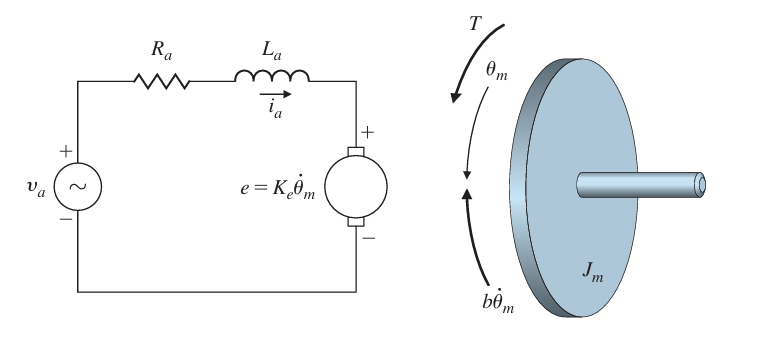
\includegraphics[width=0.7\linewidth]{images/linear_circuit_DC.png}
		\caption{Model of the DC motor \cite{DC_motor_model}}
		\label{fig:dc_motor_model}
	\end{figure}

	\begin{figure}[htbp]
		\centering
		% To-do: Insert Figure 1 from MATLAB (voltage vs time)
		\caption{Input voltage applied to both DC motors over time}
		\label{fig:voltage_time}
	\end{figure}

	\begin{figure}[htbp]
		\centering
		% To-do: Insert Figure 2 from MATLAB (omegaA and omegaB vs time)
		\caption{Measured angular velocities for motors A and B}
		\label{fig:omega_time}
	\end{figure}

	\begin{figure}[htbp]
		\centering
		% To-do: Insert Figure 3 from MATLAB (noise comparison across periods)
		\caption{Comparison of signals across periods to assess measurement noise}
		\label{fig:noise_analysis}
	\end{figure}

	\begin{figure}[htbp]
		\centering
		% To-do: Insert Figure 4 from MATLAB (measured vs simulated without filtering)
		\caption{Model validation without filtering: measured vs simulated response for motor A}
		\label{fig:validation_unfiltered}
	\end{figure}

	\begin{figure}[h]
		\centering
		% To-do: Insert Figure 5 from MATLAB (step response of sys_d1)
		\caption{Step response of the discrete-time model (unfiltered)}
		\label{fig:step_unfiltered}
	\end{figure}

	\begin{figure}[h]
		\centering
		% To-do: Insert Figure 6 from MATLAB (averaged omegaA over one period)
		\caption{Mean angular velocity for motor A averaged across all measurement periods}
		\label{fig:omega_mean}
	\end{figure}

	\begin{figure}[h]
		\centering
		% To-do: Insert Figure 7 from MATLAB (measured vs simulated with filtering)
		\caption{Model validation with filtering: measured vs simulated response for motor A}
		\label{fig:validation_filtered}
	\end{figure}

	\begin{figure}[h]
		\centering
		% To-do: Insert Figure 8 from MATLAB (step response of sys_d2)
		\caption{Step response of the discrete-time model (filtered)}
		\label{fig:step_filtered}
	\end{figure}

\end{document}
